%%%%%%%%%%%%%%%%%%%%%%%%%%%%%%%%%%%%%%%%%%%%%%%%%%%%%%%%%%%%%%%%
%                                                              %
% Tyler Bendele                                                %
% ECE351 and Section 51                                        %
% Lab 2                                                        %
% Due Date: February 1, 2022                                   %
% Introduction to user-defined functions and demonstration     %
% of various signal operations                                 %
%                                                              %
%%%%%%%%%%%%%%%%%%%%%%%%%%%%%%%%%%%%%%%%%%%%%%%%%%%%%%%%%%%%%%%%
%%% DOCUMENT PREAMBLE %%%
\documentclass[12pt]{report}
\usepackage[english]{babel}
%\usepackage{natbib}
\usepackage{url}
\usepackage[utf8x]{inputenc}
\usepackage{amsmath}
\usepackage{graphicx}
\graphicspath{{images/}}
\usepackage{parskip}
\usepackage{fancyhdr}
\usepackage{vmargin}
\usepackage{listings}
\usepackage{hyperref}
\usepackage{xcolor}
\definecolor{codegreen}{rgb}{0,0.6,0}
\definecolor{codegray}{rgb}{0.5,0.5,0.5}
\definecolor{codeblue}{rgb}{0,0,0.95}
\definecolor{backcolour}{rgb}{0.95,0.95,0.92}
\lstdefinestyle{mystyle}{
backgroundcolor=\color{backcolour},
commentstyle=\color{codegreen},
keywordstyle=\color{codeblue},
numberstyle=\tiny\color{codegray},
stringstyle=\color{codegreen},
basicstyle=\ttfamily\footnotesize,
breakatwhitespace=false,
breaklines=true,
captionpos=b,
keepspaces=true,
numbers=left,
numbersep=5pt,
showspaces=false,
showstringspaces=false,
showtabs=false,
tabsize=2
}
\lstset{style=mystyle}
\setmarginsrb{3 cm}{2.5 cm}{3 cm}{2.5 cm}{1 cm}{1.5 cm}{1 cm}{1.5 cm}
\title{Lab 2: User Defined Functions}
% Title
\author{Tyler Bendele}
% Author
\date{January 31, 2022}
% Date
\makeatletter
\let\thetitle\@title
\let\theauthor\@author
\let\thedate\@date
\makeatother
\pagestyle{fancy}
\fancyhf{}
\rhead{\theauthor}
\lhead{\thetitle}
\cfoot{\thepage}
%%%%%%%%%%%%%%%%%%%%%%%%%%%%%%%%%%%%%%%%%%%%
\begin{document}
%%%%%%%%%%%%%%%%%%%%%%%%%%%%%%%%%%%%%%%%%%%%%%%%%%%%%%%%%%%%%%%%%%%%%%%%%%
%%%%%%%%%%%%%%%
\begin{titlepage}
\centering
\vspace*{0.5 cm}
% \includegraphics[scale = 0.075]{bsulogo.png}\\[1.0 cm] % 

\begin{center}    \textsc{\Large   ECE 351 - Section \#51 }\\[2.0 cm]
\end{center}% University Name
\textsc{\Large Signals and Systems  }\\[0.5 cm] % Course 

\rule{\linewidth}{0.2 mm} \\[0.4 cm]
{ \huge \bfseries \thetitle}\\
\rule{\linewidth}{0.2 mm} \\[1.5 cm]
\begin{minipage}{0.4\textwidth}
\begin{flushleft} \large
% \emph{Submitted To:}\\
% Name\\
% Affiliation\\
%contact info\\
\end{flushleft}
\end{minipage}~
\begin{minipage}{0.4\textwidth}
\begin{flushright} \large
\emph{Submitted By :} \\
Tyler Bendele
\end{flushright}
\end{minipage}\\[2 cm]
% \includegraphics[scale = 0.5]{PICMathLogo.png}
\end{titlepage}
%%%%%%%%%%%%%%%%%%%%%%%%%%%%%%%%%%%%%%%%%%%%%%%%%%%%%%%%%%%%%%%%%%%%%%%%%%
%%%%%%%%%%%%%%%
\tableofcontents
\pagebreak
%%%%%%%%%%%%%%%%%%%%%%%%%%%%%%%%%%%%%%%%%%%%%%%%%%%%%%%%%%%%%%%%%%%%%%%%%%
%%%%%%%%%%%%%%%
\renewcommand{\thesection}{\arabic{section}}
\section{Introduction}
The goal of this lab is to practice using user-defined functions in Python.
It is also to practice the many different signal operations and functions.
Specifically we practice using the step and ramp functions to create a
graph. After learning how to do that, we practice using the different operations including time reversal, time shifting, time scaling, and
differentiation.

\section{Equations}
The equations shown below are the function used for part 1 (labeled as equation 1) 
and the function I used to draw the graph for part 2 (labeled as equation 2).
In part 3 of the lab, equation 2 is altered in order to practice different
signal operations.
\begin{equation}
y(t) = cos(t)
\end{equation}
\begin{equation}
y(t) = r(t) - r(t-3) + 5 \cdot u(t-3) - 2 \cdot u(t-6) - 2 \cdot r(t-6)
\end{equation}
\section{Methodology}
\subsection{Part 1}
For part 1 of the lab, I was mostly able to follow the example code given in the beginning with the only change needing to be made was the actual function being plotted and the time it takes place. The code for this can be seen down below.

\begin{lstlisting}[language=Python]
steps = 1e-2
t = np.arange(0, 10 + steps, steps)

def func1(t):
    y = np.zeros(t.shape)
    for i in range(len(t)):
        y[i] = np.cos(t[i])
    return y
y = func1(t)
plt.figure(figsize = (10, 7))
plt.subplot(2, 1, 1)
plt.plot(t, y)
plt.grid()
plt.ylabel('y(t)')
plt.xlabel('t')
plt.title('Part 1 graph: y = cos(t)')
\end{lstlisting}
\subsection{Part 2}
The second part of the lab was a little bit more difficult. The
method that I ended up using was defining the unit and ramp functions from the book. I then also defined a function that created
the graph for part 2, using equation 2. This code can be seen down below.
\begin{lstlisting}[language=Python]
#%% Code used for part 2 graphs
t = np.arange(-5, 10 + steps, steps)

def u(t):          #step function
    y = np.zeros(t.shape)
    for i in range(len(t)):
        if t[i] > 0:
            y[i] = 1
        else:
            y[i] = 0
    return y

def r(t):          #ramp function
    y = np.zeros(t.shape)
    for i in range(len(t)):
       if t[i] > 0:
           y[i] = t[i]
       else:
           y[i] = 0
    return y

y = u(t)   
plt.figure(figsize = (10, 7))
plt.subplot(2, 1, 1)
plt.plot(t, y)
plt.grid()
plt.ylabel('y(t)')
plt.xlabel('t')
plt.title('Part 2: Step Function')

y = r(t)   
plt.figure(figsize = (10, 7))
plt.subplot(2, 1, 1)
plt.plot(t, y)
plt.grid()
plt.ylabel('y(t)')
plt.xlabel('t')
plt.title('Part 2: Ramp Function')

def part2(t):
    z = np.zeros(t.shape)
    z = r(t) - r(t-3) + 5*u(t-3) - 2*u(t-6) - 2*r(t-6)
    return z

z = part2(t)   
plt.figure(figsize = (10, 7))
plt.subplot(2, 1, 1)
plt.plot(t, z)
plt.grid()
plt.ylabel('y(t)')
plt.xlabel('t')
plt.title('Part 2 graph')
\end{lstlisting}
\subsection{Part 3}
Because I set up equation 2 in a function, this made part 3 much easier.
I was able to edit the functions just like the lab said to do. I used a
time reversal by making the input t negative and changing the range to be
-10 to 5 instead. The process went similarly for tasks 2 and 3.
Task 5 required two derivatives and slightly different graph
changes. The rest of the code can be seen down below.
\begin{lstlisting}[language=Python]
# Time Reversal
t = np.arange(-10, 5 + steps, steps)
tr = part2(-t)
plt.figure(figsize = (10, 7))
plt.subplot(2, 1, 1)
plt.plot(t, tr)
plt.grid()
plt.ylabel('y(t)')
plt.xlabel('t')
plt.title('Time Reversal')

# Time Shift f(t-4)
t = np.arange(0, 14 + steps, steps)
ts = part2(t-4)
plt.figure(figsize = (10, 7))
plt.subplot(2, 1, 1)
plt.plot(t, ts)
plt.grid()
plt.ylabel('y(t)')
plt.xlabel('t')
plt.title('Time Shift f(t-4)')

# Time Shift f(-t-4)
t = np.arange(-14, 0 + steps, steps)
ts = part2(-t-4)
plt.figure(figsize = (10, 7))
plt.subplot(2, 1, 1)
plt.plot(t, ts)
plt.grid()
plt.ylabel('y(t)')
plt.xlabel('t')
plt.title('Time Shift f(-t-4)')

# Time Scale f(t/2)
t = np.arange(-5, 20 + steps, steps)
tsc = part2(t/2)
plt.figure(figsize = (10, 7))
plt.subplot(2, 1, 1)
plt.plot(t, tsc)
plt.grid()
plt.ylabel('y(t)')
plt.xlabel('t')
plt.title('Time Scale f(t/2)')

# Time Scale f(2t)
t = np.arange(-5, 10 + steps, steps)
tsc = part2(2*t)
plt.figure(figsize = (10, 7))
plt.subplot(2, 1, 1)
plt.plot(t, tsc)
plt.grid()
plt.ylabel('y(t)')
plt.xlabel('t')
plt.title('Time Scale f(t/2)')

# Derivative
t = np.arange(-5, 10 + steps, steps)
dt = np.diff(t)
dy = np.diff(part2(t))/dt

plt.figure(figsize = (10, 7))
plt.subplot(2, 1, 1)
plt.ylim((-2,10))
plt.plot(t[range(len(dy))], dy)
plt.grid()
plt.ylabel('y(t)')
plt.xlabel('t')
plt.title('Derivative')
\end{lstlisting}

\section{Results}
As far as I can tell I got all of the expected results.
\subsection{Part 1}
\begin{figure}[h!]
\begin{center}
\caption{Part 1, Task 2}
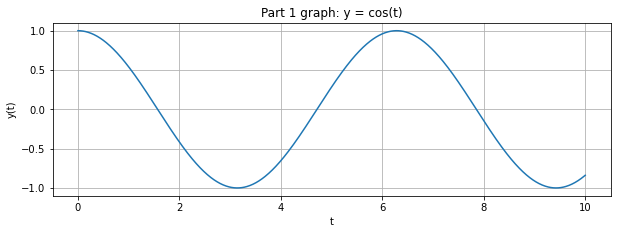
\includegraphics[scale=0.65]{Part1Task.png}
\end{center}
\end{figure}
\newpage
\subsection{Part 2} {
\begin{figure}[h!]
\begin{center}
\caption{Part 2, Task 2, Step Function}
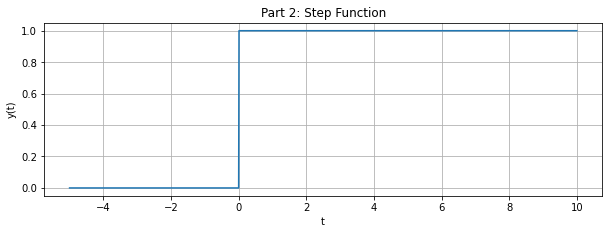
\includegraphics[scale=0.55]{Part2Step.png}
\end{center}
\end{figure}

\begin{figure}[h!]
\begin{center}
\caption{Part 2, Task 2, Ramp Function}
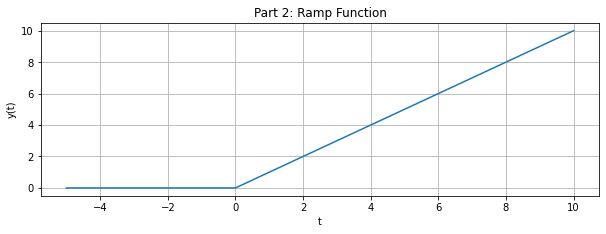
\includegraphics[scale=0.65]{Part2Ramp.png}
\end{center}
\end{figure}

\begin{figure}[h!]
\begin{center}
\caption{Part 2, Task 3, Graph}
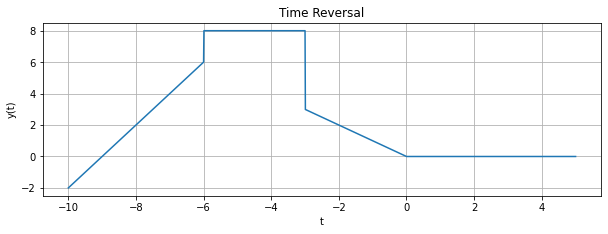
\includegraphics[scale=0.65]{Part2Task.png}
\end{center}
\end{figure}
}
\newpage
\subsection{Part 3} {
\begin{figure}[h!]
\begin{center}
\caption{Part 3, Task 1, Time Reversal}
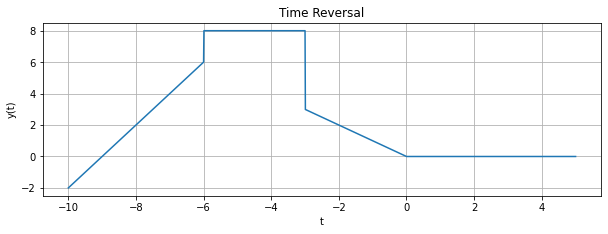
\includegraphics[scale=0.65]{Task1.png}
\end{center}
\end{figure}

\begin{figure}[h!]
\begin{center}
\caption{Part 3, Task 2-1, Time Shift}
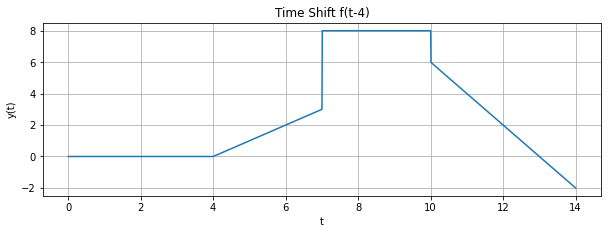
\includegraphics[scale=0.65]{Task2_1.png}
\end{center}
\end{figure}

\begin{figure}[h!]
\begin{center}
\caption{Part 3, Task 2-2, Time Shift}
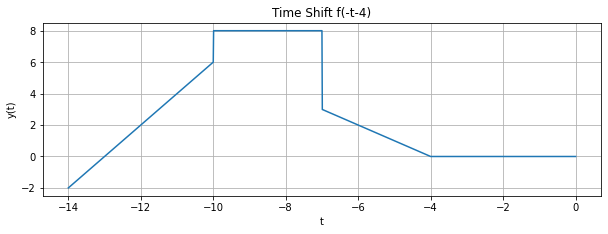
\includegraphics[scale=0.65]{Task2_2.png}
\end{center}
\end{figure}

\begin{figure}[h!]
\begin{center}
\caption{Part 3, Task 3-1, Time Scale}
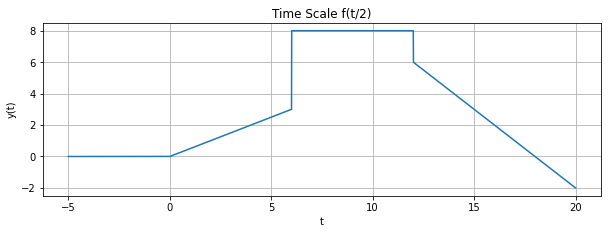
\includegraphics[scale=0.65]{Task3_1.png}
\end{center}
\end{figure}

\begin{figure}[h!]
\begin{center}
\caption{Part 3, Task 3-2, Time Scale}
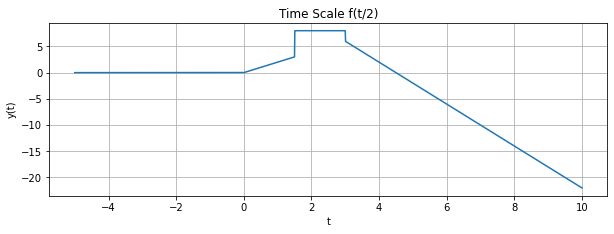
\includegraphics[scale=0.55]{Task3_2.png}
\end{center}
\end{figure}

\begin{figure}[h!]
\begin{center}
\caption{Part 3, Task 4, Hand Drawn Derivative Graph}
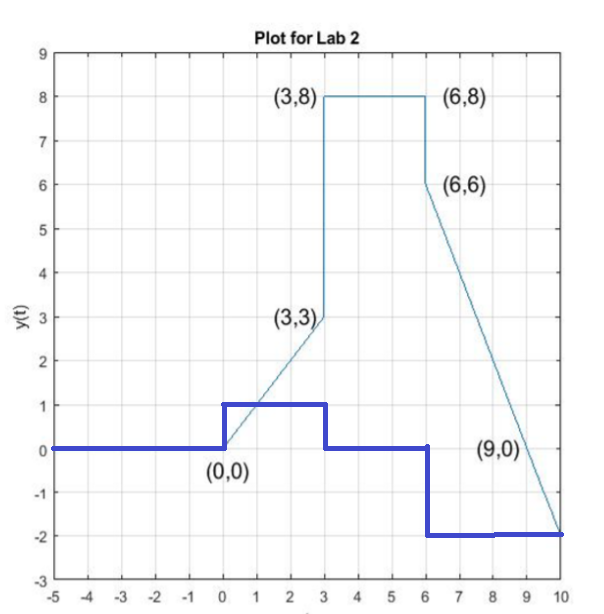
\includegraphics[scale=0.65]{DerivativePlot.png}
\end{center}
\end{figure}

\begin{figure}[h!]
\begin{center}
\caption{Part 3, Task 5, Python Derivative Plot}
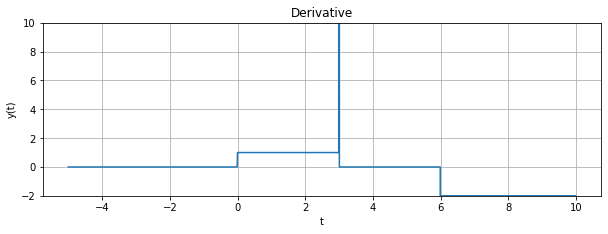
\includegraphics[scale=0.55]{Task5.png}
\end{center}
\end{figure}
}

\newpage
\newpage
\section{Error Analysis}
In the final result of the Python code, there are not any errors that I am aware of.
I did however have quite a bit of problems getting to this point of no error. The
first part of the lab went pretty smoothly. The second part of the lab is where
I started having difficulty. My first problem was that I put for loops in the
function for the third task. This added unneeded complications. I also used
t instead of t[i] in my step and ramp functions. Luckily I was able to figure
these problems out. The next major problem came with trying to do task 1 of part 3.
I tried multiple different things and wasn't getting the correct result. I ended
up realizing that I needed to change the boundaries of t for each different task.
Finally, the only other problem I had was formatting the graph for the derivative, but I
ended up figuring out good boundaries for it.

In terms of problems with \LaTeX, I couldn't figure out how to make the
pictures stay in the right spots.
\section{Questions}
1. Are the plots from Part 3 Task 4 and Part 3 Task 5 identical? Is it possible for them to
match? Explain why or why not.

They don't quite match because I graphed Task 4 on the grid of the Part 2 graph and
I didn't add the discontinuities. In general they are pretty close to matching each
other. So, I would definitely say they are possible to match because it is a
computer plot versus my own graphing skills.

2. How does the correlation between the two plots (from Part 3 Task 4 and Part 3 Task 5)
change if you were to change the step size within the time variable in Task 5? Explain why this happens.

Reading this question I realize what is meant by the first question. Unfortunately,
I forgot to add the curves at the points where there should be discontinuities. Similarly, to the step size problem in Part 1, I would expect that by making the 
step size smaller, the quality of the graph in Task 5 would more closely resemble 
curves going off to infinity at the discontinuities that look like straight lines.

3. Leave any feedback on the clarity of lab tasks, expectations, and deliverables.

I think I was confused on how the tasks were formatted when first working on the lab, 
after working on it for quite some time I think I understood what is expected. I
also believe that the deliverables are in the correct spot. On that note, I think my only question is how to fix
either the subsections or the pictures so they actually stay where I put them? I was able to put in new page commands which seemed to help a little bit, but I was wondering if there are any other ways to make it look better?

\section{Conclusion}
In this lab it seems a lot of things were brand new to me. Because of all of
these new things, I learned a load of things from this lab. I learned quite a lot about user defined functions. I also learned more about how to make graphs in
Python and how it doesn't graph correctly if you don't set the correct bounds.
Furthermore, I learned about several signal operations that can be performed on
functions and how they look when graphed. As far as recommendations go, I
think the lab was pretty clear in stating what was expected to be done in the
lab. The only recommendation I would maybe make is swapping tasks 1 and 2 on 
Part 2 and adding a little more detail on how to go about putting the 
functions together. The instructions seem pretty clear now after doing the
lab, but they were a little confusing going through it the first time. An insight that I had this lab that will affect how I do future labs, I would
say based on the amount of problems that I had that it would definitely be
beneficial for me to try and solve the problems that I have sooner rather than later.
\end{document}
%This template was created by Roza Aceska.